\chapter{Fundamentação Teórica}
\label{ch:fundamentacao}
\par Neste capítulo ser\~ao fundamentados os conhecimentos b\'asicos para o entendimento do trabalho.

\section{Java}

\par Java é uma linguagem de programação multiplataforma, concorrente (executa mais de uma tarefa em paralelo), baseada em classes e orientada a objetos \cite{joy2000java}.
\par A linguagem Java é compilada e interpretada. Após escrever um programa em Java, estes são salvos como código fonte com extensão ".java". Quando estes códigos fontes são compilados, um arquivo binário chamado de arquivo de classe com extensão ".class" é gerado. Estes arquivos não são executados diretamente pelos processadores, pois eles não contêm instruções para os mesmos. Os programas Java são compilados em um formato de arquivo chamado \textit{bytecode}. Desta forma, esses programas podem ser executados em qualquer sistema operacional que possua um interpretador JVM (Java \textit{Virtual Machine}) em um JRE (Java \textit{Runtime} \textit{Environment}) conforme Figura \ref{fig:ambiente java}. Assim, o código precisa ser compilado apenas uma vez para funcionar em qualquer sistema operacional que possua a configuração citada, pois os \textit{bytecodes} serão executados da mesma forma pela JVM \cite{arnold2005java}.

\begin{image}
{0.2}
{src/imagens/cap1/ambiente-java.png}
{Ambiente Java}{fig:ambiente java}
{Adaptado de \citeonline{javaprogrammingenvioronment2010}}
\end{image}

\par É uma linguagem fortemente tipada, isto é, as características das variáveis tem que ser definidas em tempo de compilação. Ela possui um coletor de lixo (\textit{garbage collector}) para evitar problemas de segurança como \textit{deadlock}. \cite{joy2000java}

\subsection{Reflexão}

% Magão usa \citeonline{guerra2014componentes} By: Menino
\par De acordo com \citeonline{guerra2014componentes} o conceito de reflexão pode ser definido como um processo em que um programa pode visualizar e alterar sua própria estrutura ou comportamento. As classes de reflexão disponíveis em Java localizam-se no pacote \textit{java.lang.reflect}, porém, na API (\textit{Application Programming Interface}) padrão do Java as classes deste pacote aplicam o conceito de introspecção, que é a obtenção de informações sobre sua estrutura, sem possibilidade de modificação, não existem funcionalidades de modificação disponibilizadas por padrão pela API Reflection. Com o conceito de introspecção é possível recuperar informações de acordo com o tipo atual, que são: objeto, método, anotação, interface, classe ou campo. A Figura \ref{fig:tipos-e-retornos-introspeccao} exibe os principais métodos dos tipos classe, método, objeto e atributo. 

\begin{image}
{1} %scale
{src/imagens/cap2/metodos-introspeccao.jpg} %relative path
{Principais métodos de introspecção disponíveis por tipo} %caption
{fig:tipos-e-retornos-introspeccao} %label
{\cite{parson2000using}} %font
\end{image}

\par Cada tipo citado anteriormente possui sua implementação para retornar as informações necessárias, a classe \textit{Class} possui as características da classe do objeto atual em memória, e a partir dela é possível realizar as operações de introspecção vide Figura \ref{fig:introspeccao-flow}, isto é, a classe X possui uma instância de \textit{Class} com seus metadados como seu nome, construtores, assinatura dos métodos, nome e modificadores dos atributos, existência de anotações, e assim vai suscetivamente até que a classe \textit{Class} possua uma instância com suas características.

\begin{image}
{0.4} %scale
{src/imagens/cap2/reflection-diagrama.png} %relative path
{Fluxo de reflexão para obter informações sobre instâncias} %caption
{fig:introspeccao-flow} %label
{\citeonline{guerra2014componentes}} %font
\end{image}

\par Com reflexão é possível recuperar informações padrões sobre os dados (classes, métodos e atributos), porém não é possível realizar processos mais sofisticados como validações ou alguma regra de negócio baseando-se nisto \cite{guerra2010architectural}, para este tipo de necessidade foi criado uma forma de adição de metadados em Java, para facilitar este processo que era realizado via arquivos ou recursos não padrão, esta solução foi a criação das anotações \citeonline{jcp175metadata2002facility}.

\subsubsection{\textit{Proxy} Dinâmico}

\par Para entender o conceito de \textit{proxy} dinâmico (PD), o padrão de projeto \textit{proxy} proposto por \citeonline{gamma1995design}, exibido na Figura \ref{fig:proxy-pattern} precisa ser abordado antes. Este tem como objetivo o encapsulamento de um objeto e a implementação de sua interface, ou seja, um objeto X com uma interface Y é encapsulado por um objeto Z que implementa a interface Y também, possuindo os mesmos métodos.
%Desta forma as execuções dos métodos do objeto encapsulado são interceptadas pelo \textit{proxy}. Em outras palavras, a cada chamada de métodos do objeto encapsulado, o \textit{proxy} é executado antes conforme Figura \ref{fig:proxy-pattern}.

\begin{image}
{0.2} %scale
{src/imagens/cap2/proxy-pattern-criado.png} %relative path
{Padrão de projeto \textit{proxy}} %caption
{fig:proxy-pattern} %label
{Adaptado de \cite{gamma1995design}} %font
\end{image}

%, assim processos podem ser realizados de forma transparente aos dois pontos (o cliente que invocou o método e o objeto que foi invocado). 

\par Quando o cliente (Figura \ref{fig:proxy-pattern}) realiza chamadas de métodos do assuntoReal (objeto encapsulado), estas são enviadas ao \textit{proxy} primeiramente, 
portanto, todas as execuções de métodos do objeto encapsulado são interceptadas pelo \textit{proxy}. Na execução do \textit{proxy} qualquer lógica pode ser aplicada, como validações ou chamadas de outros métodos. Ao final da execução das lógicas definidas no \textit{proxy}, a responsabilidade é devolvida ao objeto encapsulado. Um problema na utilização de \textit{proxies} é a dependência da interface, pois caso outro objeto precise ser encapsulado sua interface também precisa ser implementada, ou seja, outro \textit{proxy} deverá ser criado.

\par PD é um recurso disponibilizado pela API reflexão (\textit{reflection}) do Java, a fim de interceptar invocações de objetos de forma semelhante ao padrão de projeto \textit{proxy} apresentado na Figura \ref{fig:proxy-pattern}, entretanto sua principal diferença é que objetos com qualquer interface podem ser interceptados, devido a forma de criação do \textit{proxy} dinâmico pela JVM a partir do método estático \textit{newProxyInstance} da classe \textit{Proxy}, que devolve uma instância que será utilizada no lugar do objeto encapsulado com os parâmetros passados para este método, a Figura \ref{fig:proxy-dinamico} exemplifica o funcionamento de um \textit{proxy} dinâmico. 

\begin{image}
{0.3} %scale
{src/imagens/cap2/funcionamento-proxy-dinamico.png} %relative path
{Funcionamento do \textit{proxy} dinâmico} %caption
{fig:proxy-dinamico} %label
{\cite{guerra2014componentes}} %font
\end{image}

\par O método estático criaProxyDinamico da Figura \ref{fig:cria-proxy-dinamico} recebe um objeto como parâmetro (linha 8), e ele é encapsulado de acordo com a ideia do padrão de projeto \textit{proxy} na linha 12, a partir da criação de uma nova instância da classe atual (ProxyDinamicoExemplo). Com essa nova instância, o método construtor privado localizado na linha 4 é invocado, e nele, a referência do objeto recebido na linha 8 é encapsulada. O retorno do método criaProxyDinamico é o objeto encapsulado pelo \textit{proxy} dinâmico, a partir dos parâmetros passados para o método estático \textit{newProxyInstance}. Este recebe três parâmetros: 1) \textit{ClassLoader} do objeto; 2) Interfaces do objeto; 3) Uma instância da implementação de \textit{InvocationHandler}; O proxy dinâmico é criado com esses parâmetros pela JVM conforme já dito, e todas invocações do objeto são interceptadas pelo terceiro parâmetro passado na instância do \textit{proxy}, que é uma implementação de \textit{InvocationHandler}, neste exemplo a própria classe ProxyDinamicoExemplo.

\begin{figure}[H]
    \centering
    \caption{Criação do \textit{proxy} dinâmico}
    \label{fig:cria-proxy-dinamico}
    \begin{java}
public class ProxyDinamicoExemplo implements InvocationHandler {
    	private Object objetoEncapsulado;

	private ProxyDinamicoExemplo(Object objetoEncapsulado) {
		this.objetoEncapsulado = objetoEncapsulado;
	}
//Recupera ClassLoader e interfaces do objeto passado como parametro via reflexao
	public static <T> T criaProxyDinamico(Object object) {
		return (T) Proxy.newProxyInstance(
        		object.getClass().getClassLoader(),
        		object.getClass().getInterfaces(),
        		new ProxyDinamicoExemplo(object)
		);
	}
//Implementacao do metodo Invoker omitido
}
    \end{java}
    \fonte{Produção do autor}
\end{figure}


\par A interface \textit{InvocationHandler} do pacote \textit{java.lang.reflect} define um método apenas, o \textit{Invoke}, vide Figura \ref{fig:invoke-implementacao}, este método é executado antes de qualquer invocação do objeto encapsulado no processo anterior de criação do \textit{proxy}.

\begin{figure}[H]
    \centering
    \caption{Implementação da interface \textit{InvocationHanlder}}
\begin{java}
public class ProxyDinamicoExemplo implements InvocationHandler {
//encapsulamento do objeto e metodo de criacao do proxy omitidos
	@Override
	public Object invoke(Object proxy, Method method, Object[] args) throws Throwable {
		Class clazz = this.getClass();
		Logger.getLogger(clazz.getName())
		    .log(
                        Level.INFO, "Metodo " +
                        method.getName() + 
                        " interceptado pelo proxy dinamico " +
                        clazz.getSimpleName()
		    );
		Object resultadoDaInvocacao = method.invoke(objetoEncapsulado, args);
		return resultadoDaInvocacao;
	}
}
\end{java}
    \label{fig:invoke-implementacao}
    \fonte{Produção do autor}
\end{figure}

\par A cada invocação do objeto encapsulado, o método \textit{invoke} é executado antes, de acordo com a Figura \ref{fig:invoke-registrando-log} onde é possível verificar a criação do \textit{proxy} dinâmico na linha 4, onde o método criaProxyDinamico da Figura \ref{fig:cria-proxy-dinamico} é chamado, retornando um \textit{proxy} do tipo \textit{Executor}, este possui o método \textit{executionTime} que retorna uma instância de \textit{java.util.Date}.

\begin{figure}[H]
    \centering
    \caption{Registros da invocação interceptada}
    \label{fig:invoke-registrando-log}
    \begin{java}
public class App {
	public static void main(String[] args) {
	
		Executor executor = ProxyDinamicoExemplo.criaProxyDinamico(new ExecutandoProxyDinamico());
		System.out.println(executor.executionTime());
	}
}
    \end{java}
    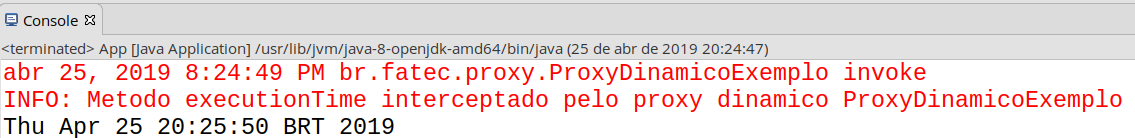
\includegraphics[scale=0.4]{src/imagens/cap2/invoke-registrando-log.png}
    \fonte{Produção do autor}
\end{figure}

Quando o PD é invocado, logs são criados conforme linha 6 da Figura \ref{fig:invoke-implementacao}, esta linha exibe o método interceptado e nome do \textit{proxy}. Sempre que o objeto \textit{executor} (objeto encapsulado) for invocado, um log será gerado.

\subsection{Anotação}

\par Anotações em Java, são utilizadas para definição de metadados, isto é, informações sobre algo, estas podem ser inseridas em: Pacotes; Classes; Interfaces; Métodos; Atributos; Parâmetros; Construtores; e em Anotações \cite{jcp2005annotation269}. O local onde uma anotação pode ser inserida é definido pela anotação \textit{@Target} que recebe de um a N parâmetros do Enum tipo \textit{java.lang.annotation.ElementType}\footnote{É interessante restringir o local onde as anotações podem ser inseridas para evitar uma má interpretação durante sua recuperação via reflexão}, a Tabela \ref{tab:targets} exibe os parâmetros disponíveis e seu escopo. Quando uma anotação é inserida fora de seu escopo um erro de compilação com a mensagem \textit{"The annotation @NomeDaAnotação is disallowed for this location"} \citeonline{joy2000java}.

\begin{table}[H]
    \centering
    \caption{Parâmetros e restrições de anotações}
    \begin{tabular}{|l|l|}
        \hline
        Parâmetro & Escopo \\ \hline
        TYPE & Classes, Enums, Anotações, Interfaces e  Pacotes \\ \hline
        FIELD & Atributos \\ \hline
        METHOD & Métodos \\ \hline
        PARAMETER & Parâmetros \\ \hline
        CONSTRUCTOR & Construtores \\ \hline
        LOCAL\_VARIABLE & Variáveis locais (dentro de métodos) \\ \hline ANNOTATION\_TYPE & Anotações \\ \hline
        PACKAGE & Pacotes \\ \hline
        TYPE\_PARAMETER  & Tipos genéricos definidos em Métodos, Classes e Interfaces \\ \hline
        TYPE\_USE & Variáveis com tipos genéricos \\ \hline
\end{tabular}
    \label{tab:targets}
    \fonte{Adaptado de Java specification}
\end{table}

Definido o escopo de atuação da anotação é preciso definir seu escopo de duração, isto é, até onde ela será mantida no código, pois as anotações não são persistidas até o tempo de execução sem uma anotação chamada \textit{@Retention}. Esta define o ciclo de vida da anotação, na Tabela \ref{tab:retentions} seus parâmetros, que são de um a N Enum do tipo \textit{java.lang.annotation.RetentionPolicy} são explicados \citeonline{joy2000java}.

\begin{table}[H]
    \centering
    \caption{Parâmtros da anotação retention e seu tempo de duração}
    \begin{tabular}{|l|l|} \hline
        Parâmetro & Ciclo de vida\\ \hline
        SOURCE    & Anotações não são carregadas nos arquivos ".class"\\ \hline
        CLASS     & \begin{tabular}[c]{@{}l@{}}
        Anotações são mantidas nos arquivos ".class" \\mas não são carregados pela JVM
        \end{tabular} \\ \hline
        RUNTIME   & Anotações são mantidas pelos arquivos ".class" e carregados pela JVM \\ \hline
    \end{tabular}
    \label{tab:retentions}
    \fonte{Adaptado de Java specification}
\end{table}

\par O parâmetro \textit{SOURCE} é utilizado geralmente por IDE's (\textit{Integrated Development Environment}), para adicionar algum comportamento específico como a anotação \textit{@SuppressWarnings} que serve para ignorar algum aviso, presente em IDE's como o Eclipse e o IntelliJ IDEA. Para que uma anotação seja recuperada em tempo de execução é preciso adicionar a \textit{RetentionPolicy Runtime}, devido ao comportamento padrão da anotação \textit{@Retention} que é o valor \textit{CLASS} \cite{joy2000java}.

\par É possível adicionar propriedades em uma anotação para complementar comportamentos ou informações que esta proporcionará, as propriedades permitidas são: Tipos primitivos; Enums; Class (Apenas a classe Class); String; Anotações; e Arrays dos tipos anteriores conforme Figura \ref{fig:propriedades-anotacoes}.

\begin{figure}[H]
    \centering
    \caption{Propriedades permitidas em anotações}
    \begin{java}
Anotacao anotacoes();
Class classes();
String strings();
boolean boleanos();
byte bytes();
char chars();
double doubles();
float floats();
int inteiros();
long longs();	
short shorts();
Anotacao[] arrayDeAnotacoes();
Class[] arrayDeClasses();
String[] arrayDeStrings();
boolean[] arrayDeBoleanos();
byte[] arrayDeBytes();
char[] arrayDeChars();
double[] arrayDeDoubles();
float[] arrayDeFloats();
int[] arrayDeInteiros();
long[] arrayDeLongs();	
short[] arrayDeShorts();
    \end{java}
    \label{fig:propriedades-anotacoes}
    \fonte{Adaptado de \cite{joy2000java}}
\end{figure}

\par Na Figura \ref{fig:declaracao-anotacao} uma anotação é declarada para exemplificação, esta é mantida até o tempo de execução e pode ser adicionada em outras anotações e métodos. Por padrão, nenhum comportamento é adicionado ou alterado com a adição de uma anotação, isto é feito a partir de métodos que verificam sua existência, como reflexão citada no capítulo anterior \cite{bloch2004jsr}. 

\begin{figure}[H]
    \centering
    \caption{Declaração de uma anotação}
    \begin{java}
@Target({ ANNOTATION_TYPE, METHOD })
@Retention(RUNTIME)
public @interface Anotacao {
}
    \end{java}
    \label{fig:declaracao-anotacao}
    \fonte{Produção do autor}
\end{figure}

\textit{Frameworks} baseados em reflexão e metadados são \textit{softwares} que utilizam a reflexão para obtenção de metadados, estes disponibilizam anotações com o valor \textit{Runtime} para sejam lidos posteriormente \cite{guerra2009pattern}.

\section{\textit{Framework}}

\par Um \textit{framework} é considerado um \textit{software} incompleto que é especializado com o comportamento de uma aplicação externa \cite{johnson1988designing}. Este determina a arquitetura que a aplicação utilizará, sua organização, como: convenções de nomes, arquitetura do projeto, arquivos externos de configuração e/ou anotações. Isto é definido para que o desenvolvedor tenha que se preocupar apenas com o problema que está resolvendo. A forma que o \textit{framework} realiza esta organização deve ser baseada no que é mais viável para solucionar a situação comum em relação ao problema encontrado, permitindo que a tarefa repetitiva ou específica seja reaproveitada em novos projetos.
Baseado nisso \textit{frameworks} permitem que aplicações com estruturas semelhantes sejam criadas, facilitando a manutenção, padronização e legibilidade do código, entretanto, isto restringe o desenvolvedor a solução que o \textit{framework} aplica, não permitindo que determinados caminhos sejam seguidos ou certas decisões sejam tomadas no projeto \cite{gamma2009padroes}. A ideia por trás dessa restrição citada é a inversão de controle existente, onde os \textit{frameworks} chamam o código que foi desenvolvido, não o contrário, desta forma muitas vezes é realizada a injeção de dependências neste código criado, que é o fornecimento de implementações de interfaces em tempo de execução, a Figura \ref{fig:inversao-controle} exemplifica uma situação em que existe a inversão de controle em um ambiente Web, onde a requisição é recebida pelo servidor e a responsabilidade inicial é do framework, este realiza o processamento inicial passando a requisição por filtros e outras validações e depois passa a responsabilidade para as classes criadas pelo desenvolvedor final.

\begin{image}
{0.18} %scale
{src/imagens/cap2/arquitetura-spring-traduzida.png} %relative path
{Inversão de controle} %caption
{fig:inversao-controle} %label
{Adaptado de \citeonline{spring-mvc-architecture}} %font
\end{image}

\par Existem pontos extensíveis em frameworks, estes são chamados de \textit{hotspots} e servem para especializações como no exemplo anterior (Figura \ref{fig:inversao-controle}) em que os blocos roxos são os hotspots fornecidos. Estes são implementados pelos desenvolvedores pois é possível atender requisitos como filtros genéricos que precisam ser verificados e restrições recuperadas de metadados, porém funcionalidades específicas não tem como serem atendidas em todos os caos, e precisam ser implementadas via hotspots, geralmente frameworks disponibilizam algumas especializações prontas para hostspots, mas caso seja necessário outras podem ser criadas para situações em que as soluções existentes não resolverem o problema. Por outro lado, ao contrário dos hotspots existem os frozenspots (blocos azuis da Figura \ref{fig:inversao-controle}) que são trechos que não devem ser alterados ou especializados de formas diferentes, são as funcionalidades e processos automatizados pelo framework \cite{markiewicz2001object}

\subsection{Frameworks baseados em Reflexão e Metadados}

\par \textit{Frameworks} baseados em metadados revolucionaram a ideia do desenvolvimento destas soluções, devido ao problema da limitação de expressão que existia. Era possível adicionar comportamentos no \textit{framework} via implementações de interfaces, heranças de classes abstratas (\textit{hook methods}), definição programática e arquivos externos de configuração. Convenções de nome como \textit{getters} e \textit{setters} dos Java \textit{Beans} por exemplo, são formas de adição de metadado que podem ser utilizados por \textit{frameworks} quando estes possuem algum valor semântico, a Figura \ref{fig:spring-qyery-method} exibe como \textit{query methods} são utilizados pelo Spring JPA, nele os parâmetros de consulta são inseridos no nome do método e o SQL é criado em tempo de execução, o Spring identifica que a interface possui \textit{query methods} com a extensão de interfaces parametrizadas em sua documentação, estas são: Repository, CrudRepository e JpaRepository. Definições programáticas são limitadas e quando é necessário expressar informações mais complexas, a criação de metadados com esta abordagem não é viável.

\begin{figure}[H]
    \centering
    \caption{Query method Spring JPA}
    \begin{java}
public interface CrudRepository<T, Integer> {
    Optional<T> findById(Integer id);
}
    \end{java}
    \label{fig:spring-qyery-method}
    \fonte{\citeonline{gierke_darimont_strobl_paluch_bryant_2019}}
\end{figure}

Arquivos externos são muito verbosos pois precisam descrever precisamente onde as modificações acontecerão ou onde estão agregando informações, a Figura \ref{fig:arquivo-metadado} exibe um arquivo de configuração básica de persistência de uma entidade para o Hibernate.

\begin{figure}[H]
    \centering
    \caption{Configuração de persistência de uma classe via XML}
    \begin{xml}
<?xml version="1.0"?>
<!DOCTYPE hibernate-mapping PUBLIC "-//Hibernate/Hibernate Mapping DTD 3.0//EN"
"http://hibernate.sourceforge.net/hibernate-mapping-3.0.dtd">

<hibernate-mapping>
    <class name="br.fatec.sjc.exemplo.Pessoa" table="pessoa" catalog="exemplo">
        <id name="pessoaId" type="java.lang.Integer">
            <column name="PES_ID" />
            <generator class="identity" />
        </id>
        <property name="nome" type="string">
            <column name="PES_NOME" length="50" not-null="true" unique="false" />
        </property>
        <property name="cpf" type="string">
            <column name="PES_CPF" length="11" not-null="true" unique="true" />
        </property>
    </class>
</hibernate-mapping>
    \end{xml}
    \label{fig:arquivo-metadado}
    \fonte{Adaptado de \cite{xml-hibernate-configuration}}
\end{figure}

\par Para resolver estes problemas as anotações foram criadas conforme JCP 269 \citeonline{jcp2005annotation269}. Com as anotações os metadados são inseridos no próprio código, deixando a semântica mais fluída e menos verbosa. Na Figura \ref{fig:classe-metadado} é realizada a mesma configuração da Figura \ref{fig:arquivo-metadado}, neste exemplo é possível analisar a facilidade que as anotações trouxeram para o desenvolvimento, possibilitando que metadados sejam adicionados de uma forma mais natural, fazendo parte da própria linguagem.

\begin{figure}[H]
    \centering
    \caption{Configuração de persistência de um classe via anotação}
    \begin{java}
@Entity
@Table(name = "pessoa", uniqueConstraints = { @UniqueConstraint(columnNames = { "cpf" }) 
})
public class Pessoa implements Serializable {

	@Id
	private Integer id;
	@Column(nullable = false)
	private String nome;
	@Column(nullable = false)
	private String cpf;

    // Getters e setters omitidos

}
    \end{java}
    \label{fig:classe-metadado}
    \fonte{Adaptado de \citeonline{annotation-configuration-hibernate}}
\end{figure}

O uso de anotações é chamado de programação orientada a atributos \cite{buschmann2007pattern}, com a adição desta nova funcionalidade adição de metadados complexos é possível, a leitura destes também é facilitada pois as anotações fazem partes da API, assim os problemas citados nesta seção foram solucionados.

\section{Gamificação}

\par Gamificação pode ser definido como a utilização de conceitos de design de jogos, como: Ganho de pontos, \textit{ranking}, troféus, e \textit{rewards} em aplicações de outros contextos \cite{deterding2011gamification}. \textit{Softwares} de e-commerce, sites de e-learning, são alguns exemplos de contextos onde a gamificação pode ser aplicada. Um exemplo de aplicação que utiliza gamificação é a Foldit \cite{burke2012behind}, que utiliza conceitos de pontos e troféus em um jogo de quebra cabeça, para na verdade, prever a estrutura da proteína humana \cite{deterding2011gamification}. O propósito da gamificação é fazer com que a utilização das aplicações não diminua com o tempo e proporcione experiências melhores ao usuário, pois as conquistas adquiridas durante a utilização incentivam a continuidade. A Psicologia Comportamental trata desta abordagem utilizada na gamificação como reforços positivos e negativos \cite{skinner1990behavior}. Os reforços positivos tem como objetivo estimular indivíduos a repetirem ações a partir da agregação de algo, na gamificação isto é aplicado com a ideia da aquisição das conquistas, e como já dito, isto estimula o indivíduo a continuar os processos que está fazendo para receber mais conquistas. Por outro lado, existem os reforços negativos, que incentivam o indivíduo a realizar o processo inverso do que foi feito para receber este estimulo, isto é, o comportamento é condicionado a partir de processos para evitar alguma situação, como por exemplo perder pontos ou perder posições no ranking se tratando de gamificação, isto gera efeitos colaterais como fuga e esquiva no indivíduo e este aprende naturalmente a evitar reforços negativos \cite{linehan2015gamification}. Nas duas formas é possível condicionar o indivíduo a realizar atividades para chegar a um propósito.

\section{Esfinge Project}

\par Esfinge Project\footnote{O projeto está disponível no endereço: http://esfinge.sf.net.} é um projeto \textit{open-source} iniciado em 2011 por Dr. Eduardo Guerra junto a GSW, que tem como objetivo a criação de soluções reutilizáveis para um desenvolvimento ágil, um produto final flexível e de fácil manutenção.
\par O projeto disponibiliza 9 frameworks até o momento, estes são: QueryBuilder, Comparison, Guardian, AOM Role Mapper, SystemGlue, Gamification, Metadata, Classmock, ReTest.
\par Todos os frameworks citados acima seguem uma filosofia que consiste em: Configuração de metadados para que o comportamento desejado ocorra; Componentes que podem ser integrados a aplicações de forma simples; Pontos de extensão para criação de novas funcionalidades; Remover a preocupação com a solução que o framework disponibiliza, permitindo que o desenvolvedor foque apenas em sua aplicação específica \citeonline{esfingeproject2011}.

\subsection{Esfinge Gamification}

\par O Esfinge Gamification\footnote{A documentação do projeto está disponível no endereço: http://esfinge.sourceforge.net/Gamification.html.} é um \textit{framework} que aplica lógica gamificação para \textit{softwares} que necessitam destes processos. Independente do domínio do \textit{software} é possível utilizar o \textit{framework}, pois este é desacoplado de lógicas da aplicação, sua responsabilidade é a tratativa dos dados de gamificação, portanto, pode ser integrado a qualquer programa Java, permitindo que o desenvolvedor foque na solução que está trabalhando, e deixe as responsabilidades de gamificação para o \textit{framework}  \citeonline{esfingegamification2011}.

%conforme Figura \ref{fig:esfinge-gamification-plugado}
%\begin{figure}[H]
%    \centering
%    \caption{Diagrama de %atuação do Esfinge %Gamification}
%    \label{fig:esfinge-ga%mification-plugado}
%\end{figure}

\par O comportamento do \textit{framework} é especificado via metadados conforme a filosofia dos projetos Esfinge citada anteriormente, estes são anotações que podem ser adicionada em programas Java, a Tabela \ref{tab:anotacoes-gamification} detalha as opções disponíveis. Existem quatro tipos de processos implementados pelo \textit{framework}, estes são: Ponto, Ranking, \textit{Reward}, Troféu vide Figura \ref{fig:arquitetura-esfinge-gamification}.

\begin{table}[H]
\caption{Anotações disponibilizadas pelo Esfinge Gamification}
\resizebox{\textwidth}{!}{
\begin{tabular}{|l|l|}
\hline
Anotação & Comportamento \\ \hline
\begin{tabular}[c]{@{}l@{}}@PointsToUser, @RankingsToUser, \\ @RewardsToUser, @TrophiesToUses\end{tabular} & Incremento de conquista para o usuário atual. \\ \hline
\begin{tabular}[c]{@{}l@{}}@RemoveRankings, @RemovePoints, \\ @RemoveReward, @RemoveTrophy\end{tabular} & Eliminação de conquista do usuário atual. \\ \hline
\begin{tabular}[c]{@{}l@{}}@PointToParam, @RankingToParam,\\ @RewardToParam, @TrophyToParam\end{tabular} & \begin{tabular}[c]{@{}l@{}}Incremento de conquistas para outro usuário, \\ ou seja, a ação do usuário logado no sistema \\ gera pontos para outro usuário.\end{tabular} \\ \hline
@RemovePointsToParam & \begin{tabular}[c]{@{}l@{}}Remove Pontos de outro usuário seguindo a \\ lógica de atribuição, isto é, o usuário que está\\ logado no sistema desencadeia este comportamento.\end{tabular} \\ \hline
@TrophyWhenReachPointLimit & \begin{tabular}[c]{@{}l@{}}Cria um EventListener para adicionar\\ troféus quando uma quantidade de \\ Pontos for alcançada.\end{tabular} \\ \hline
\end{tabular}
}
    \label{tab:anotacoes-gamification}
    \fonte{Adaptado de \citeonline{esfingegamification2011}}
\end{table}

\begin{image}
{1} %scale
{src/imagens/cap2/estrutura-conquistas.png} %relative path
{Conquistas implementadas no projeto Esfinge Gamification} %caption
{fig:arquitetura-esfinge-gamification} %label
{\citeonline{esfingegamification2011}} %font
\end{image}

\subsubsection{Características das conquistas disponibilizadas}

\par Ponto: Tem como intenção atribuir determinada quantidade de pontos e seu tipo, por exemplo, uma conquista que atribui 10 pontos de moedas de ouro, onde moedas de ouro são o tipo e 10 os pontos atribuídos. 
\par Ranking: Se assemelha a uma hierarquia militar, onde o ranking é de status, não de posições. Por exemplo, um usuário possui o status iniciante quando começa a utilizar a aplicação, e quando realiza algum processo específico, é premiado com o status de intermediário ou avançado.

\par Troféu: Pode ser atribuído uma vez apenas, por exemplo, caso um usuário realize um processo e receba um troféu por isto, na próxima vez que realizar o mesmo processo não receberá outro troféu.

\par \textit{Reward}: É uma conquista que é consumida, ou seja fica indisponível após ser usada. Por exemplo, um \textit{reward} de bônus de ligações será recebido não consumido por padrão, só será consumido quando uma ligação for realizada com seu recurso de bônus.

\subsubsection{Pontos de extensão}

O \textit{framework} possui dois pontos de extensão (\textit{hotspots}), onde novos comportamentos podem ser adicionados quando necessário. Desta forma é possível aplicar outras lógicas de gamificação, implementando a interface \textit{Achievement} (Figura \ref{fig:arquitetura-esfinge-gamification}) disponível no pacote \textit{net.sf.esfinge.gamification.achievement}, caso os comportamentos disponibilizados pelo \textit{framework} não sejam adequados \`a determinada situação. 
\par A interface \textit{Achievement} exibida na Figura \ref{fig:interface-achievement} possuí três métodos, eles servem para realizar os respectivos processos em \textit{Achievements}: Recuperação de nome; Incrementar informações (adição de pontos por exemplo); e remoção.

\begin{figure}[H]
    \centering
    \caption{Interface \textit{Achievement}}
    \begin{java}
public interface Achievement {
    
	public String getName();

	public void incrementAchievement(Achievement a);

	public boolean removeAchievement(Achievement r);
}
    \end{java}
    \label{fig:interface-achievement}
    \fonte{Produção do autor}
\end{figure}

\par Implementando esta interface novas ações podem ser adicionados via anotações, elas possuirão a anotação @GamificationProcessor exibida na Figura \ref{fig:gamification-processor}, que recebe uma classe que implemente a interface \textit{AchievementProcessor} como parâmetro.

\begin{figure}
    \centering
    \caption{Anotação \textit{@GamificationProcessor}}
    \begin{java}
// anotacoes retention e target omitidas
public @interface GamificationProcessor {
	Class<? extends AchievementProcessor> value();
}

    \end{java}
    \label{fig:gamification-processor}
\end{figure}

\par A Figura \ref{fig:points-to-user} exemplifica a anotação @PointsToUser, que possui a classe \textit{PointsToUserProcessor} (Figura \ref{fig:achievement-processor-implementado}) como implementação de \textit{AchievementProcessor}. Cada anotação criada possuirá uma implementação de \textit{AchievementProcessor} que executa o comportamento específico da anotação, isto é, a anotação adiciona a informação e o \textit{AchievementProcessor} seu comportamento.

%A Figura \ref{fig:bpmn-buscando-metadados} exibe como é realizada a busca desses metadados... a estrutura das anotações, utilizando como exemplo a anotação @PointsToUser, e a Figura \ref{fig:achievement-processor-implementado} exibe como é o comportamento deste metadado.

\begin{figure}[H]
    \centering
    \caption{Anotação \textit{@PointsToUser}}
    \begin{java}
// anotacoes target e retention omitidas
@GamificationProcessor(PointsToUserProcessor.class)
public @interface PointsToUser {	
	int quantity();
	String name();
}
    \end{java}
    \label{fig:points-to-user}
    \fonte{Adaptado de \citeonline{esfingegamification2011}}
\end{figure}

\begin{figure}[H]
    \centering
    \caption{Implementação de \textit{AchievementProcessor} que define comportamento da anotação \textit{@PointsToUser}}
\begin{java}
public class PointsToUserProcessor implements AchievementProcessor {
	
	private int quantity;
	private String name;

	@Override
	public void receiveAnnotation(Annotation an) {
		PointsToUser ptu = (PointsToUser) an;
		quantity = ptu.quantity();
		name = ptu.name();
	}

	@Override
	public void process(Game game, Object encapsulated, Method method, Object[] args) {
		Object user = UserStorage.getUserID();
		Point p = new Point(quantity, name);
		game.addAchievement(user, p);
	}
}
    \end{java}
    \label{fig:achievement-processor-implementado}
    \fonte{Adaptado de \citeonline{esfingegamification2011}}
\end{figure}

\par A interface \textit{AchievementProcessor} exibida na Figura \ref{fig:achievement-processor} possui dois métodos a serem implementados, estes são: \textit{receiveAnnotation} e \textit{process}. Eles tem o objetivo de recuperar informações da anotação recebida e executar seu comportamento, respectivamente. A Figura \ref{fig:achievement-processor-implementado} exibe um exemplo onde as informações \textit{quantity} e \textit{name} são recuperadas da anotação \textit{@PointsToUser} entre as linhas 8 e 10. O comportamento desta implementação é a atribuição de pontos, portanto o método \textit{addAchievement} é invocado para que isso seja persistido de acordo com a especialização da classe \textit{Game}.

\begin{figure}[H]
    \centering
    \caption{Interface \textit{AchievementProcessor}}
    \begin{java}
public interface AchievementProcessor {
	
	public void receiveAnnotation(Annotation an);
	
	public void process(Game game, Object encapsulated, Method method, Object[] args);

}
    \end{java}
    \label{fig:achievement-processor}
\end{figure}

Também é possível adicionar novos comportamentos de persistência estendendo a classe abstrata \textit{Game}, disponível no pacote \textit{net.sf.esfinge.gamification.mechanics}. Atualmente existem três implementações, estas são: Persistência em arquivo de propriedades; Banco de dados relacional; e em memória \cite{esfingegamification2011}.

\subsubsection{Funcionamento do Esfinge Gamification}

\par A Figura \ref{fig:gamification-diagrama-classe-cap2} apresenta o diagrama de classe do projeto, já o diagrama apresentado na Figura \ref{fig:diagrama-funcionamento-gamification} exibe o fluxo de funcionamento do Esfinge Gamification. A classe \textit{UserStorage} possui dois métodos, \textit{setUserID} e \textit{getUserID}, responsáveis por definir o usuário que será utilizado nos processos de gamificação e recuperar este usuário, respectivamente.

\begin{image}
{0.33} %scale
{src/imagens/cap2/gamification-class-diagram-cap2.png} %relative path
{Diagrama de classes do projeto Esfinge Gamification} %caption
{fig:gamification-diagrama-classe-cap2} %label
{Produção do autor} %font
\end{image}

\begin{image}
{0.5} %scale
{src/imagens/cap2/bpmn-gamification.png} %relative path
{Fluxo de funcionamento do Esfinge Gamification} %caption
{fig:diagrama-funcionamento-gamification} %label
{Produção do autor} %font
\end{image}

\par O método estático \textit{createProxy} da classe \textit{GameProxy} é responsável pela criação de um \textit{proxy} dinâmico que inicia a execução do Esfinge Gamification. É possível analisar na Figura \ref{fig:gamification-proxy} que a estrutura utilizada pelo \textit{framework} é semelhante a Figura \ref{fig:cria-proxy-dinamico}. O diferencial são as validações realizadas entre as linhas 18 e 23, pois, se durante a criação alguma inconsistência nos metadados for encontrada, como as anotações @PointsToUser e  @RemovePoints no mesmo local\footnote{@PointsToUser atribui pontos e @RemovePoints remove pontos vide Tabela \ref{tab:anotacoes-gamification}}, a exceção \textit{GamificationConfigurationException} do pacote \textit{net.sf.esfinge.gamification.exception} é lançada. 

\begin{figure}[H]
    \centering
    \caption{Criação de \textit{proxy} dinâmico do Esfinge Gamification}
    \begin{java}
public class GameProxy implements InvocationHandler {
        private Object encapsulated;

	private GameProxy(Object encapsulated) {
		this.encapsulated = encapsulated;
        }
        
//implementacao do metodo invoke omitida
    
	public static <T> T createProxy(T encapsulated) {
		Object obj = Proxy.newProxyInstance(
		        encapsulated.getClass().getClassLoader(),
			encapsulated.getClass().getInterfaces(), 
			new GameProxy(encapsulated)
		);

		try {
			MetadataValidator.validateMetadataOn(
			    encapsulated.getClass()
			);
			for (Class interf : encapsulated.getClass().getInterfaces()) {
				MetadataValidator
				.validateMetadataOn(interf);
			}
		} catch (AnnotationValidationException e) {
			throw new GamificationConfigurationException("Invalid annotation configuration", e);
		}

		return (T) obj;
	}
}
    \end{java}
    \label{fig:gamification-proxy}
    \fonte{Produção do autor}
\end{figure}

A Figura \ref{fig:bpmn-recuperacao-achievement-processor} detalha os processos macro da Figura \ref{fig:diagrama-funcionamento-gamification}. Quando o \textit{proxy} intercepta execuções, este procura por metadados na classe e no método que foi interceptado, como é possível identificar no segundo passo do processo \textit{getAnnotations}. %Em outras palavras este método procura as anotações citadas na Tabela \ref{tab:anotacoes-gamification} e retorna uma lista com implementações da interface \textit{AchievementProcessor}.
Cada anotação encontrada é passada para o processo \textit{createAchievementProcessor} que procura pelos metadados citados na Tabela \ref{tab:anotacoes-gamification} retornando um \textit{Optional} com a implementação de \textit{AchievementProcessor} caso o metadado possua a anotação \textit{@GamificationProcessor} ou vazio caso não possua, para que este seja adicionado a uma lista de \textit{AchievementProcessors} criada para que os métodos \textit{process} sejam executados, aplicando o comportamento específico das anotações.

\begin{image}
{0.45} %scale
{src/imagens/cap2/bpmn-recuperacao-achievement-processor.png} %relative path
{Processo de recuperação de metadados} %caption
{fig:bpmn-recuperacao-achievement-processor} %label
{Produção do autor} %font
\end{image}

%\begin{figure}[H]
%    \centering
%    \caption{Método \textit{getAnnotations} da classe \textit{GameInvoker}}
%    \begin{java}
%public class GameInvoker {
%//restante da implementacao da classe omitida
%    private List<AchievementProcessor> getAnnotations(Method method) throws InstantiationException, IllegalAccessException {
%		List<AchievementProcessor> apList = new ArrayList<>();
%		//procura metadados no metodo
%		for(Annotation an : method.getAnnotations()){
%			createAchievementProcessor(an).ifPresent(ap -> apList.add(ap));	
%		}
		
%		//procura metadados na classe
%		for(Annotation an : method.getClass().getAnnotations()){
%			createAchievementProcessor(an).ifPresent(ap -> apList.add(ap));	
%		}
%		return apList;
%	}
%}    
%    \end{java}
%    \label{fig:buscando-metadados-game-invoker}
%\end{figure}

%Se nenhuma anotação for encontrada, o fluxo de execução é devolvido para a aplicação, entretanto, se alguma for encontrada, ela possuirá a anotação @GamificationProcessor, que recebe uma classe como parâmetro. Este é uma implementação da interface \textit{AchievementProcessor}, a Figura \ref{fig:exemplo-gamificationprocess} exemplifica a anotação @PointsToUser, que possui a classe \textit{PointsToUserProcessor} como implementação de \textit{AchievementProcessor}.

%\begin{figure}[H]
%    \centering
%    \caption{Anotação %\textit{PointsToUser}}
%    \begin{java}
%//anotacoes retention, target e Esfinge Metadata omitidas
%@GamificationProcessor(PointsToUserProcessor.class)
%public @interface PointsToUser {	
%//propriedades omitidas
%}
%    \end{java}
%    \label{fig:exemplo-gamificationprocess}
%\end{figure}


%A Figura \ref{fig:criacao-achievement-processors} exibe como é feita a busca e a recuperação das implementações da interface \textit{AchievementProcessor} presentes nos metadados. O
%método \textit{getAnnotations} exibido na Figura \ref{fig:buscando-metadados-game-invoker} invoca o 
%método \textit{createAchievementProcessor} da classe \textit{GameInvoker} nas linhas 7 e 12, passando como parâmetro as anotações recuperadas via reflexão nas linhas 6 e 11, que retornam os metadados do método e classe, respectivamente. 

%\par Na linha 5 da Figura \ref{fig:criacao-achievement-processors} o tipo da anotação é recuperado, para que nas linhas 6 e 7 a presença da anotação @GamificationProcessor seja verificada. Se a anotação for encontrada ela é recuperada com o método \textit{getAnnotation} da classe \textit{Class} nas linhas 8 e 9. Como exemplificado na Figura \ref{fig:exemplo-gamificationprocess} a anotação @GamificationProcessor recebe uma classe como parâmetro, esta é recuperada na linha 10 da Figura \ref{fig:criacao-achievement-processors}, a partir da propriedade \textit{value} da anotação @GamificationProcessor. Possuindo a classe que implementa a interface \textit{AchievementProcessor} é possível criar uma nova instância desta, e isto é realizado na linha 11 com o método \textit{newInstance} da classe \textit{Class}. Esta instância é devolvida na linha 13 para a lista de \textit{AchievementProcessor}, existente na linha 4 da Figura \ref{fig:buscando-metadados-game-invoker}.

%\begin{figure}[H]
%    \centering
%    \caption{Método \textit{createAchievementProcessor} da classe \textit{GameInvoker}}
%    \begin{java}
%public class GameInvoker{
%//restante da implementacao da classe omitida
%    private Optional<AchievementProcessor> createAchievementProcessor(Annotation an) throws InstantiationException,
%    			IllegalAccessException {
%		Class<? extends Annotation> anType = an.annotationType();
%		if(anType.isAnnotationPresent(
		    %GamificationProcessor.class)){
		%	GamificationProcessor gp = anType
		%	.getAnnotation(GamificationProcessor.class);
		%	Class<? extends AchievementProcessor> c = gp.value();
		%	AchievementProcessor ap = c.newInstance();		%		
		%	ap.receiveAnnotation(an);
		%	return Optional.of(ap);
		%}
		%return Optional.empty();
	%}
%}
%    \end{java}
%    \label{fig:criacao-achievement-processors}
%\end{figure}

%\par Para consolidar o que foi explicado, o diagrama exibido na Figura detalha o fluxo de execução dos métodos \textit{getAnnotations} e \textit{createAchievementProcessor}.

%\par Cada anotação possui uma implementação de \textit{AchievementProcessor}. Essas implementações invocam os métodos adequados da classe  \textit{Game} para as situações, por exemplo a anotação @PointsToUser invoca o método \textit{addAchievement} da classe \textit{Game} para atribuir os pontos ao usuário. Após a finalização do processamento realizado pela especialização da classe \textit{Game}, o fluxo de execução é retornado para a aplicação conforme diagrama da Figura.

\subsection{Esfinge Guardian}

\par Autorização em \textit{software} pode ser resumida na pergunta: "Esta entidade pode acessar este recurso?" \cite{sandhu1994access}. Onde entidade pode ser definida como um usuário ou sistema externo com a intenção de realizar um processo em um ambiente controlado, e recurso como algo que está sob proteção, algo não publico \cite{bartsch2011authorization}.
\par O Esfinge Guardian é um \textit{framework} para a aplicação de autorizações em \textit{softwares}, seguindo a filosofia do Esfinge Project citada anteriormente. Este aplica os seguintes modelos de controle de acesso:

\begin{itemize}
    \item \textit{Attribute Based Access Control} (ABAC): É um controle de acesso lógico que verifica atributos de objetos, em um determinado ambiente e assunto, para validar se o objeto poderá ou não realizar o acesso naquela situação baseado nas politicas definidas \cite{hu2015attribute}.
    
    \item \textit{Mandatory access control} (MAC): É um controle de acesso que é definido por apenas uma entidade no sistema, e apenas esta entidade pode realizar a alteração das permissões definidas, geralmente este tipo de controle de acesso é utilizado para informações sensíveis, é semelhante a um sistema militar \cite{lindqvist2006mandatory}.
    \item \textit{Role Based Access Control} (RBAC): É uma forma de controle de acessos baseado em funções, isto é, cada objeto (este podendo ser um usuário ou um ativo), possui uma ou mais funções que o permitem realizar determinados processos de acordo com seu nível hierárquico, semelhante a uma empresa \cite{sandhu2000nist}.
\end{itemize}

\subsubsection{Arquitetura}

\par O \textit{framework} é dividido por módulos, estes possuem a arquitetura exibida na Figura \ref{fig:arquitetura-guardian}. Abaixo seus módulos serão explicados:

\begin{itemize}
    \item \textit{Guardian}: Este é o Super POM \citeonline{apachesoftwarefoundation2019} do projeto, tem como objetivo controlar as dependências compartilhadas e o processo de empacotamento dos demais
    
    \item \textit{Guardian-core}: Tem as funcionalidades essenciais para um modelo de autorização, este modulo é utilizado por todos os modelos de controle de acesso presentes no Esfinge \textit{Guardian}.
    
    \item \textit{RBAC}, \textit{ABAC} e \textit{MAC}: Implementam os modelo de controle de acesso com seus nomes.
 
\end{itemize}

\begin{image}
{0.2} %scale
{src/imagens/cap2/arquitetura-modulos-guardian.png} %relative path
{Arquitetura dos módulos existêntes no Esfinge Guardian} %caption
{fig:arquitetura-guardian} %label
{Adaptado de \citeonline{guerra2017approach}} %font
\end{image}

\subsubsection{Pontos de extensão}

\par Nesta seção os \textit{hotspots} do Esfinge Guardian serão abordados, para estender o \textit{framework} é necessário implementar as interfaces \textit{Populator} e \textit{Authorizer}, além da criação de anotações de segurança.

\par A interface \textit{Populator} exibida na Figura \ref{fig:interface-populator} possui o método \textit{populate}, que é dedicado a recuperação de informações de segurança necessárias para a autorização. 

\begin{figure}[H]
    \centering
    \caption{Interface \textit{Populator}}
    \begin{java}
public interface Populator {
	void populate(AuthorizationContext context);
}
    \end{java}
    \label{fig:interface-populator}
    \fonte{Adaptado de \citeonline{esfingeguardian}}
\end{figure}

\par Além de implementar a interface \textit{Populator} é preciso configurá-la. Atualmente existem duas formas de realizar esta configuração, com a anotação @PopulatorClass ou com o arquivo de configuração chamado \textit{"org.esfinge.guardian.populator.Populator"}. A anotação @PopulatorClass exibida na Figura \ref{fig:populator-class} possui uma propriedade onde o \textit{Populator} implementado é definido para ser recuperado pelo \textit{framework} (linha 3).

\begin{figure}[H]
    \centering
    \caption{Anotação \textit{PopulatorClass}}
    \begin{java}
//anotacoes retention e target omitidas
public @interface PopulatorClass {
	Class<? extends Populator> value();
}
    \end{java}
    \label{fig:populator-class}
    \fonte{Adaptado de \citeonline{esfingeguardian}}
\end{figure}

\par O arquivo de configuração \textit{org.esfinge.guardian.populator.Populator} precisa estar localizado no caminho \textit{META-INF/services/} para ser identificado pelo \textit{framework}. O conteúdo deste arquivo é a classe e o pacote que implementam a interface \textit{Populator}, portanto, se a classe \textit{PopulatorImpl} localizada no pacote \textit{br.org.fatec} for configurada desta forma, o conteúdo do arquivo será \textit{br.org.fatec.PopulatorImpl} e a estrutura de diretórios ficará com o diretório META-INF localizado no mesmo nível dos pacotes, conforme a Figura \ref{fig:populator-tree} exemplifica.

\begin{image}
{0.3} %scale
{src/imagens/cap2/populator-tree.png} %relative path
{Estrutura de diretórios para identificação da implementação da interface \textit{Populator}} %caption
{fig:populator-tree} %label
{Produção do autor} %font
\end{image}

\par A interface \textit{Authorizer} (Figura \ref{fig:interface-authorizer}) possui o método \textit{authorize}, seu retorno é um booleano, que consiste na liberação da autorização ou não. Esta também possui a declaração de um atributo genérico \textit{E extends Annotation}, neste atributo é esperado a anotação de segurança que será avaliada pela implementação. 

\begin{figure}[H]
    \centering
    \caption{Interface \textit{Authorizer}}
    \begin{java}
public interface Authorizer<E extends Annotation> {
	Boolean authorize(AuthorizationContext context, E securityAnnotation);
}
    \end{java}
    \label{fig:interface-authorizer}
    \fonte{Adaptado de \citeonline{esfingeguardian}}
\end{figure}

\par As anotações de segurança precisam conter a anotação @AuthorizerClass (Figura \ref{fig:anotacao-authorizer-class}), que recebe uma classe que estenda \textit{Authorizer} como parâmetro.

\begin{figure}[H]
    \centering
    \caption{Anotação \textit{AuthorizerClass}}
    \begin{java}
//anotacoes retention e target omitidas
public @interface AuthorizerClass {
	Class<? extends Authorizer<? extends Annotation>> value();
}

    \end{java}
    \label{fig:anotacao-authorizer-class}
    \fonte{Adaptado de \citeonline{esfingeguardian}}
\end{figure}

\par A Figura \ref{fig:anotacao-seguranca} exemplifica como novas anotações de segurança devem ser implementadas.

\begin{figure}[H]
    \centering
    \caption{Exemplo de implementação da anotação \textit{AuthorizerClass}}
    \begin{java}
@Target({ ElementType.METHOD, ElementType.ANNOTATION_TYPE, ElementType.TYPE })
@Retention(RetentionPolicy.RUNTIME)
@AuthorizerClass(AnotacaoSegurancaAuthorizer.class) 
public @interface AnotacaoSeguranca { 
}
    \end{java}
    \label{fig:anotacao-seguranca}
\end{figure}

\subsubsection{Funcionamento do Esfinge Guardian}
%\par O \textit{proxy} dinâmico do Esfinge Guardian é criado a partir do método estático \textit{guardObject} da classe \textit{AuthorizationContext} que centraliza o contexto de autorização utilizado pelo \textit{framework}

\par O funcionamento do \textit{framework} pode ser visualizado no diagrama exibido na Figura \ref{fig:diagrama-funcionamento-guardian}, que tem como objetivo esclarecer o fluxo do diagrama de classes da Figura \ref{fig:guardian-diagrama-classe-cap2}. O diagrama de sequencia (Figura \ref{fig:diagrama-funcionamento-guardian}) tem como inicio a interceptação de métodos. Quando o \textit{framework} é executado, um contexto de autorização nomeado \textit{AuthorizationContext} é criado, este contexto contém informações sobre o objeto interceptado vide Figura \ref{fig:guardian-diagrama-classe-cap2}, além de informações que são utilizadas posteriormente para que a autorização ocorra. Após a criação do contexto de autorização, ele é invocado e o processamento da autorização é inciado (execução de \textit{AuthorizationProcessor}). Para que este processamento aconteça, primeiro é preciso encontrar as implementações da interface \textit{Populator}, pois elas possuem as informações necessárias para realização da autorização conforme já dito. Com as implementações encontradas, as autorizações podem ser verificadas a partir da chamada dos \textit{Authorizers} recuperados dos metadados definidos no método interceptado. Estes realizam as verificações necessárias, e caso alguma seja falsa ou falhe, a exceção \textit{AuthorizationException} do pacote \textit{org.esfinge.guardian.exception} é lançada, retornando a mensagem de erro \textit{"Unauthorized Access"}, ou caso nenhuma inconsistência ou erro sejam encontrados, é permitido que o método acesse o recurso desejado inicialmente.

\begin{landscape}

\begin{figure}
    \centering
    \caption{Diagrama de funcionamento do projeto Esfinge Guardian}
    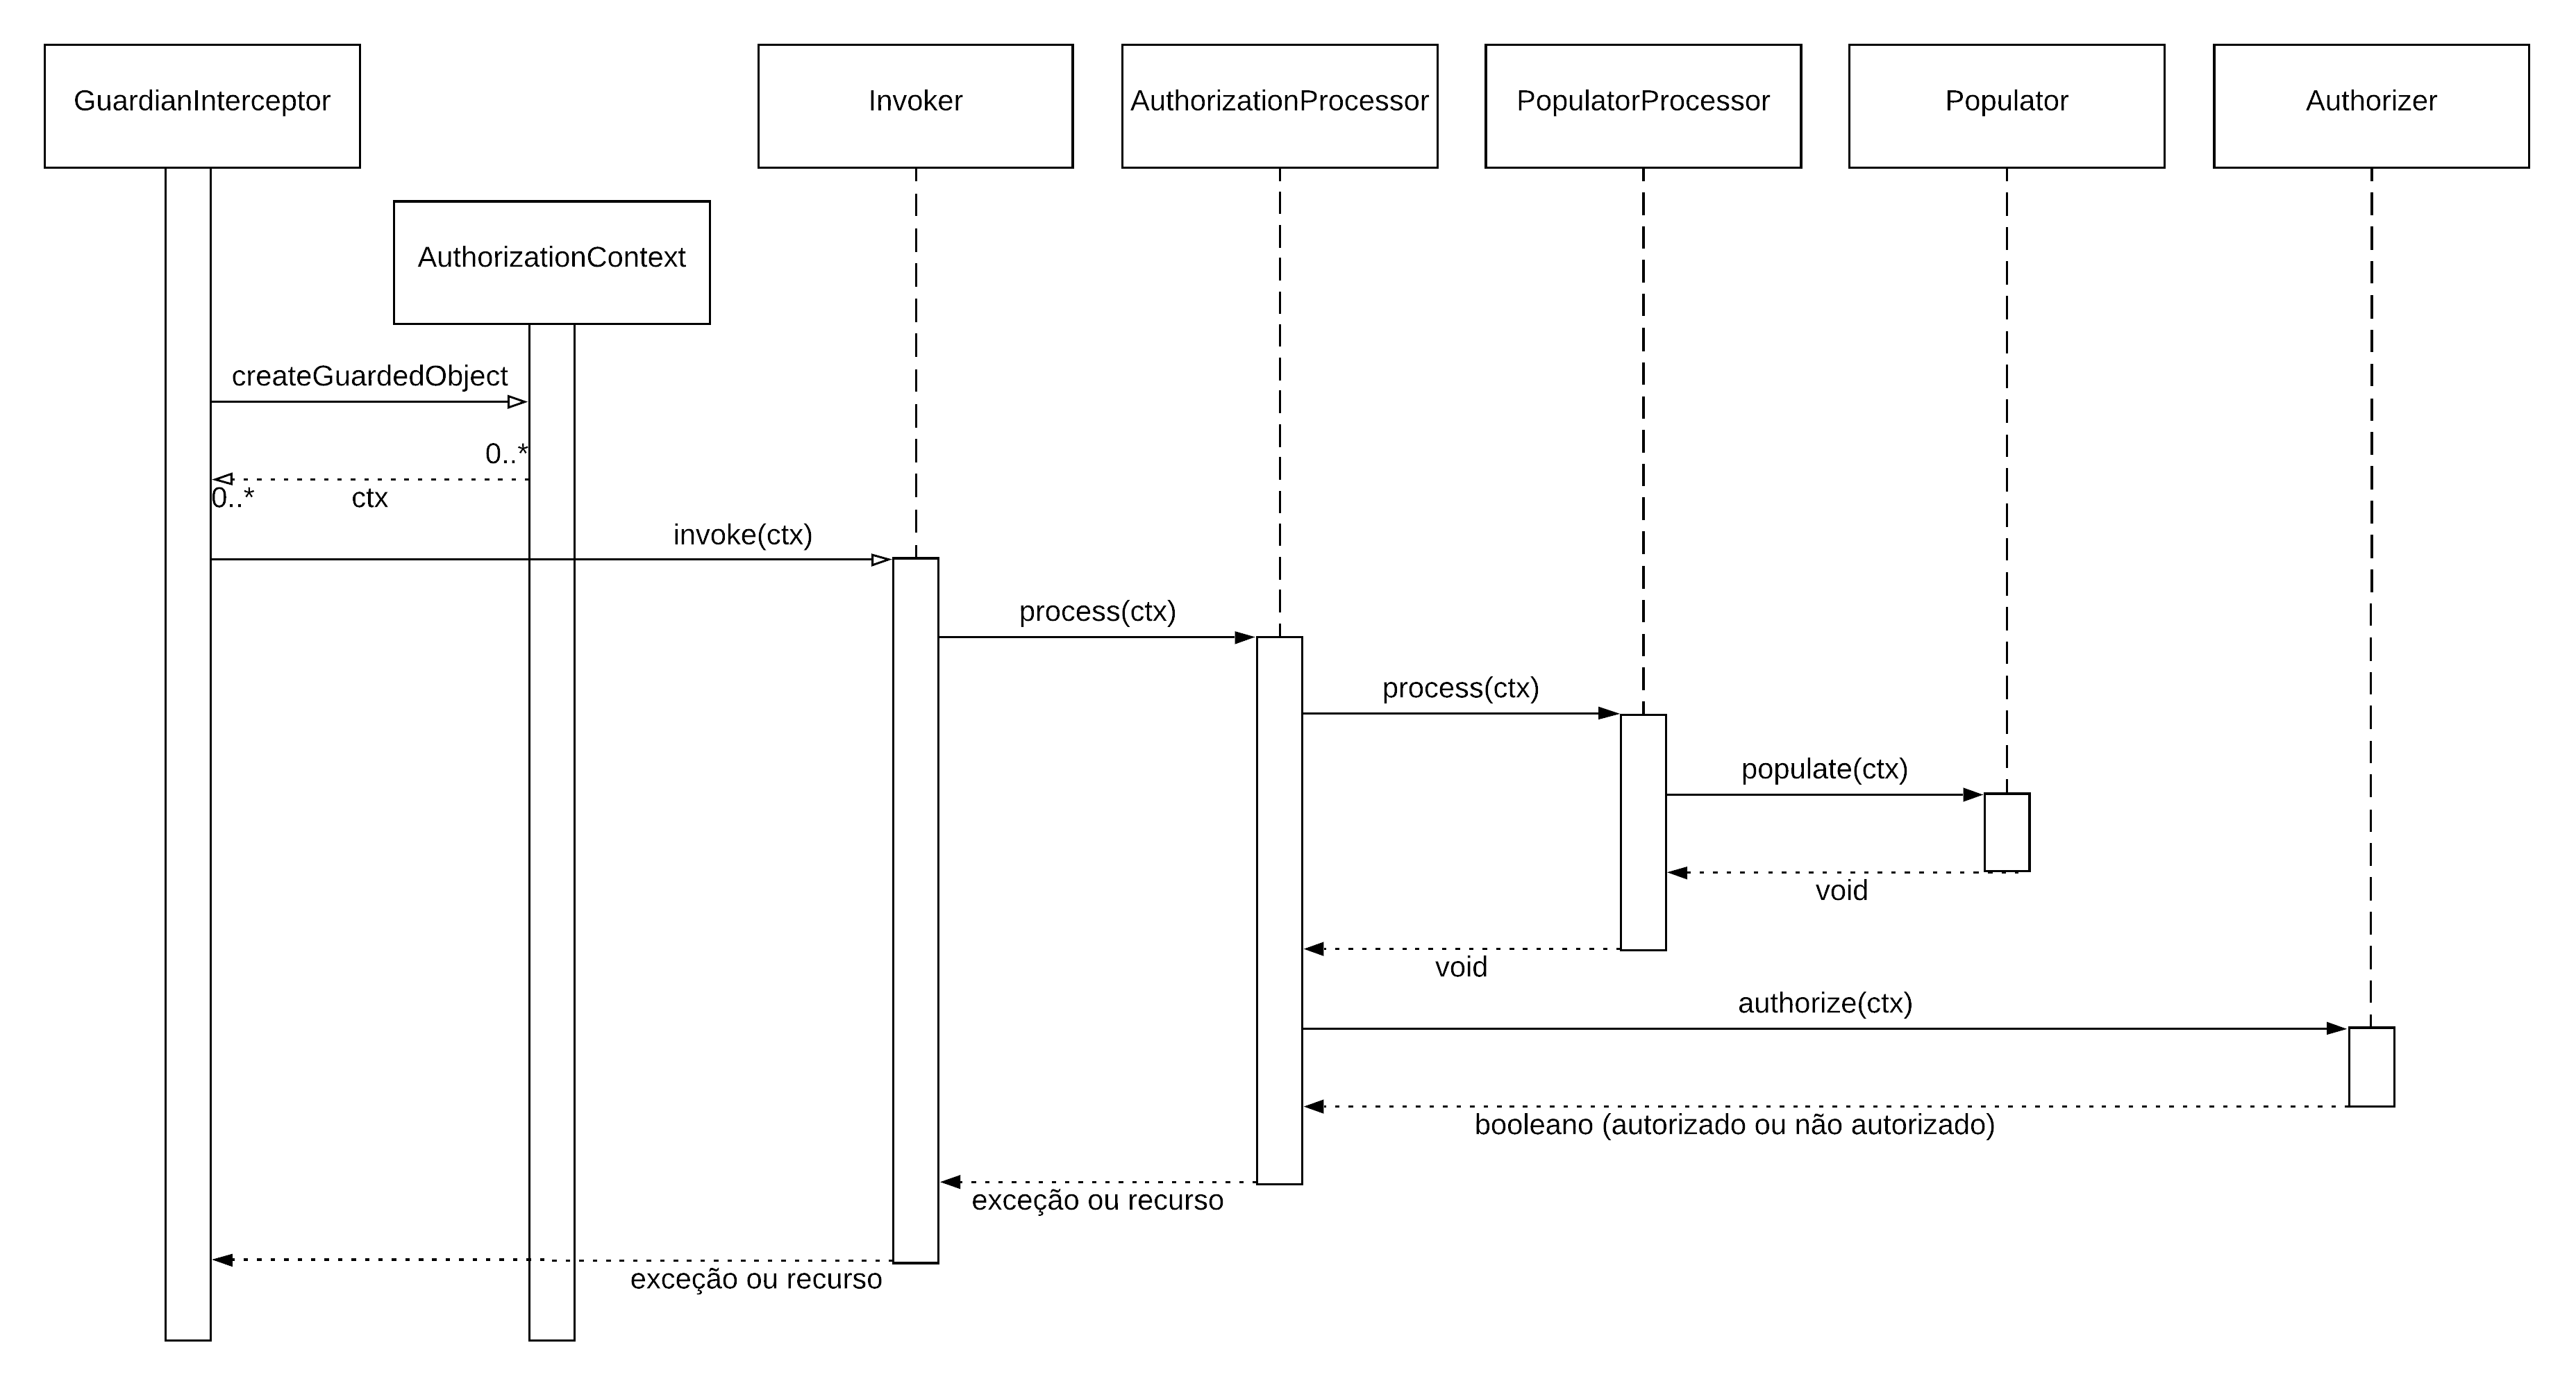
\includegraphics[scale=0.2]{src/imagens/cap2/sequencia-guardian.png}
    \label{fig:diagrama-funcionamento-guardian}
    \fonte{Produção do autor}
\end{figure}

\begin{figure}
    \centering
    \caption{Diagrama de classes do projeto Esfinge Guardian}
    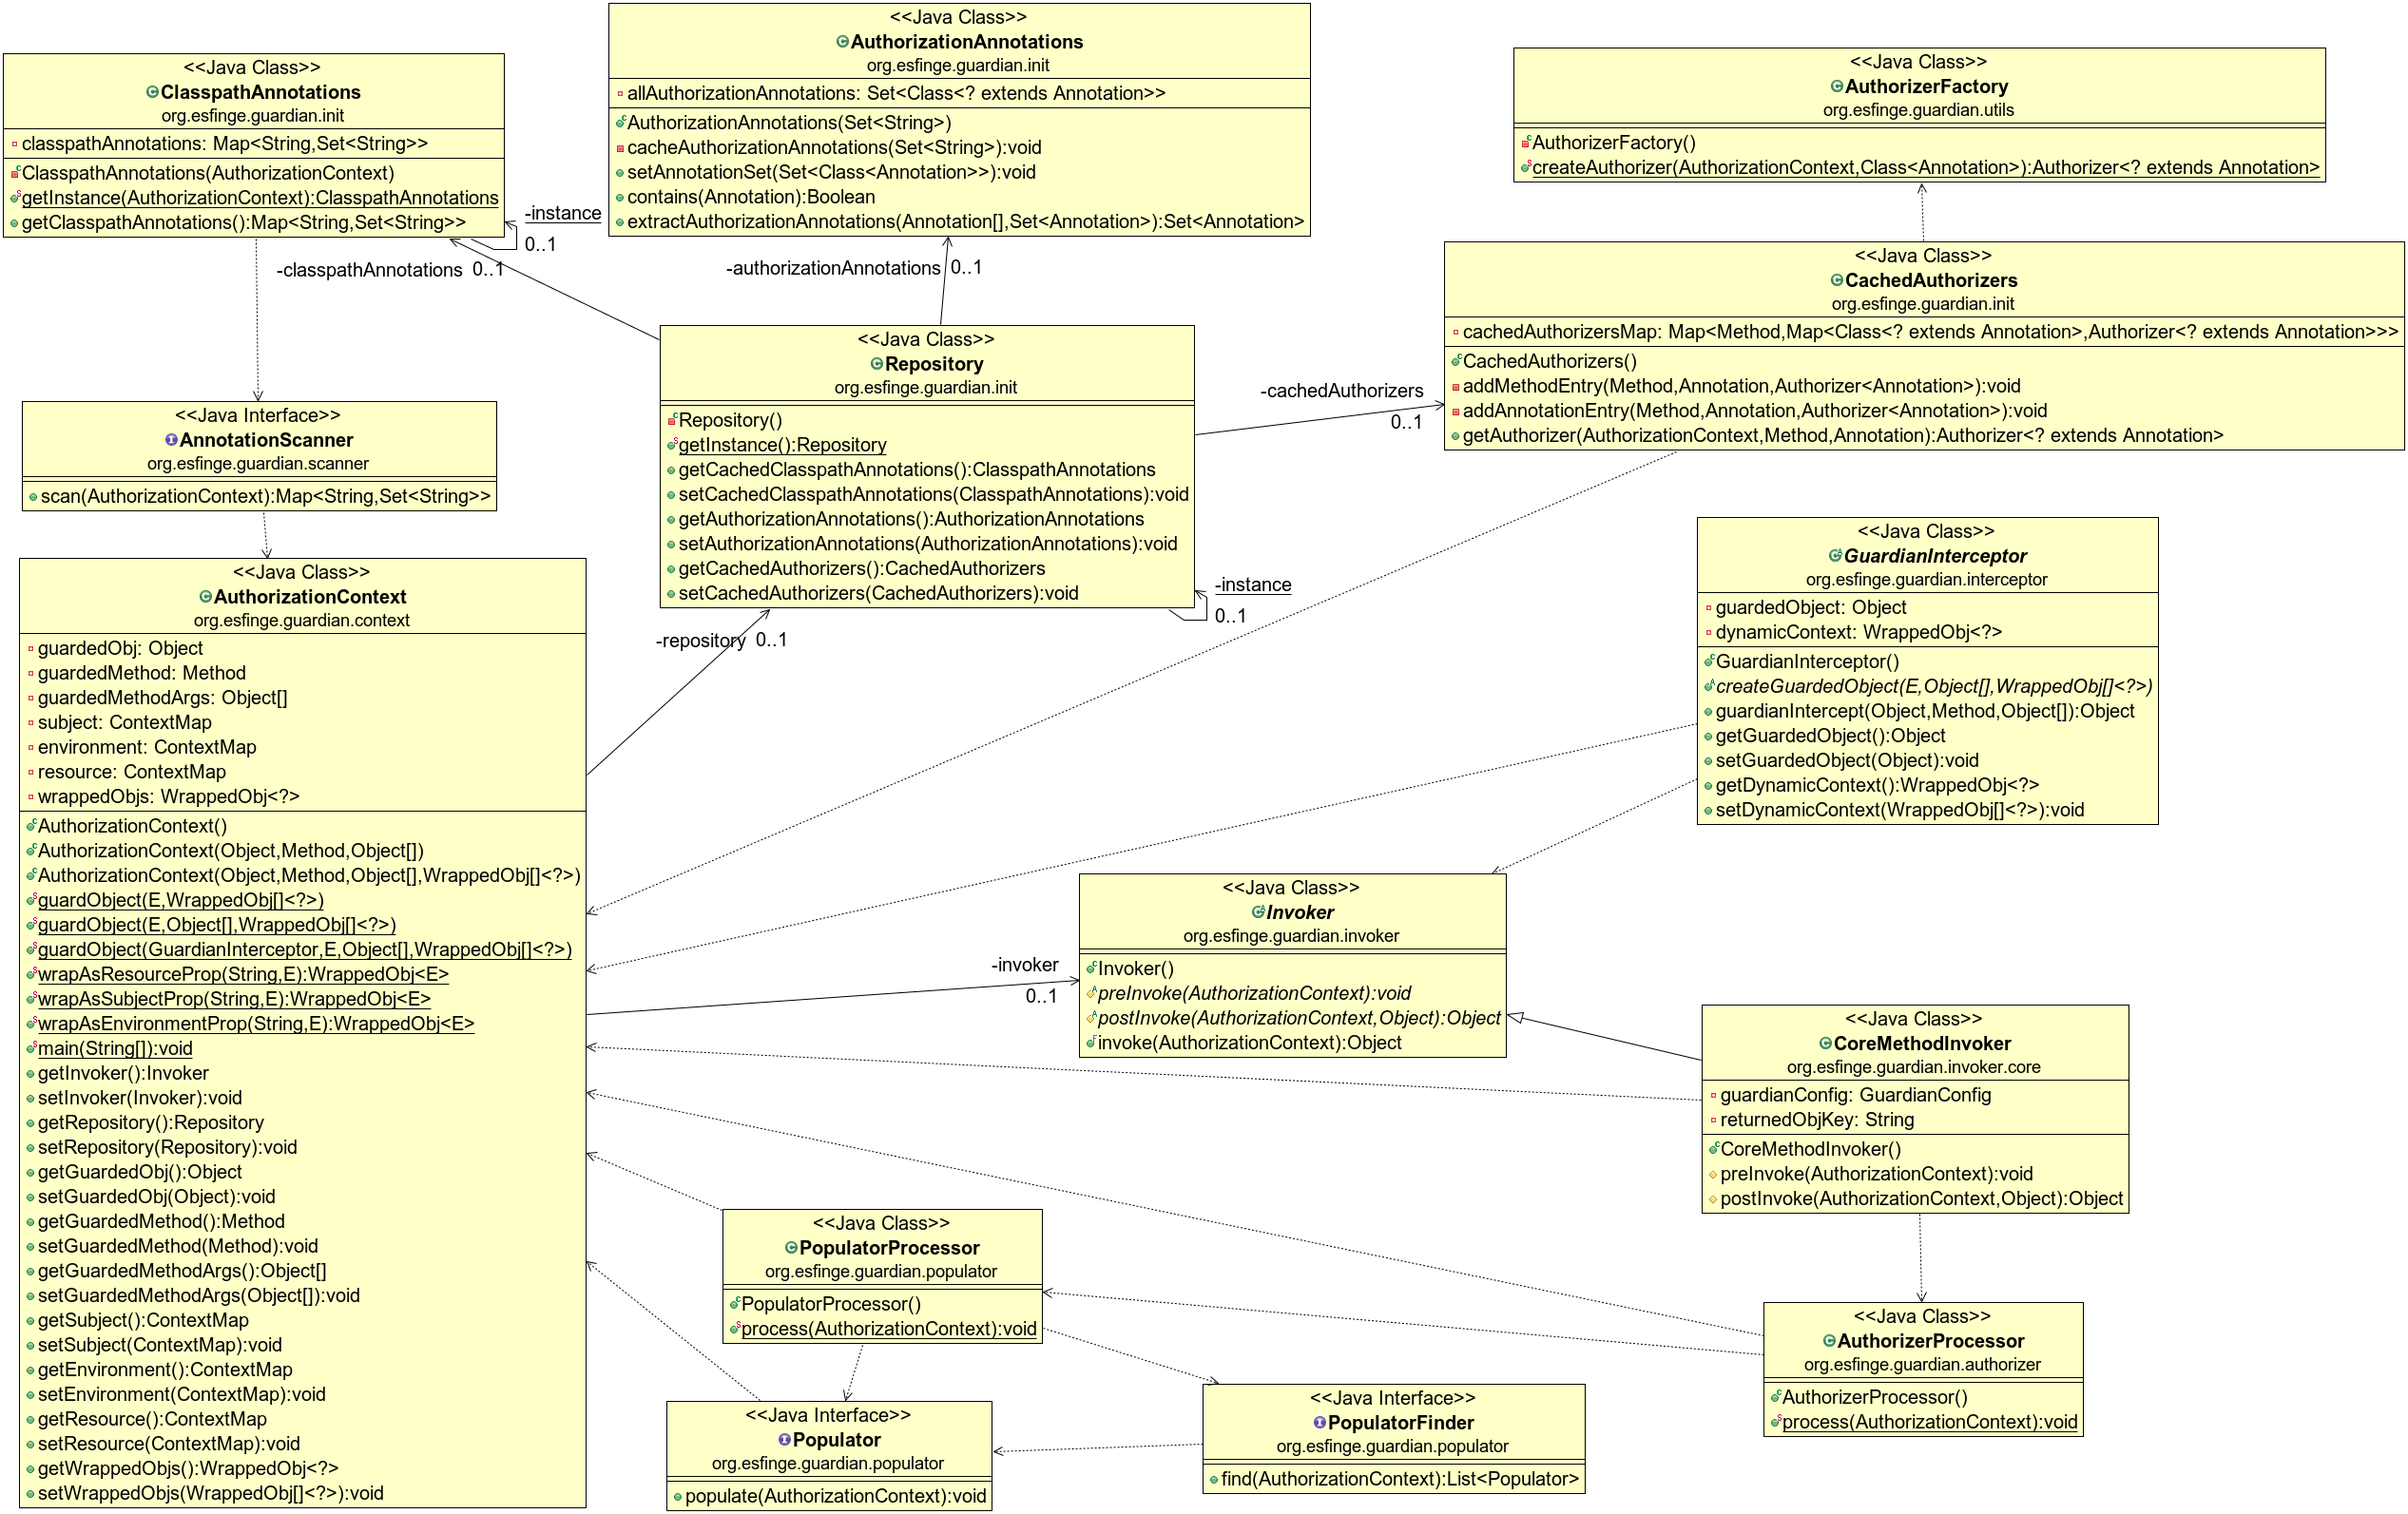
\includegraphics[scale=0.26]{src/imagens/cap2/guardian-core-class-diagram.png}
    \label{fig:guardian-diagrama-classe-cap2} %label
    \fonte{Produção do autor} %font
\end{figure}

\end{landscape}
